Questo capitolo verifica le ipotesi H2 e H3 e studia il comportamento di STERA quando i pesi si avvicinano al limite della memoria disponibile. I kernel che operano sulle coordinate sono descritti nel \autoref{cap:capitoli/04d-motore}. Descriviamo prima l'impostazione dei benchmark, poi la banda di lettura del disco, il peso dei modelli, il confronto fra i due motori dello stesso STERA 30M, l'inferenza dei tre modelli del confronto linguistico e infine l'esecuzione con pesi che superano la memoria. Per leggere i risultati distinguiamo il time to first token (TTFT), che include l'elaborazione del prompt, il decode, cioè la produzione dei token successivi, e il tempo totale della richiesta.

\section{Impostazione dei benchmark sul modello addestrato}
\label{sec:sistemi-impostazione}

\paragraph{Hardware.} Tutte le misure di inferenza della tesi sono state effettuate su un MacBook Air con chip Apple M1, 16 GiB di memoria unificata e SSD interno. Si distinguono la dimensione dei pesi persistenti e la memoria fisica occupata dall'intero processo: non sono grandezze intercambiabili.

\paragraph{Unico checkpoint STERA.} Il modello linguistico allenato è soltanto \textbf{STERA 30M}, con \num{30346182} parametri compatti e \num{82721280} elementi nella rappresentazione densa equivalente. Per isolare l'effetto dei motori, viene confrontato il percorso MLX/Metal che utilizza direttamente le coordinate con quello che carica le matrici densi ricostruite dallo stesso insieme di pesi. Tutti i test con tale coppia eseguono la medesima funzione appresa, e la coincidenza dei token generati è stata controllata sui prompt misurati.

\paragraph{Riferimenti pubblici.} Per le prove applicative sono eseguiti esclusivamente TinyStories-8M e TinyStories-33M, in due modi: con il runtime standard PyTorch/MPS con cui sono distribuiti e con un motore denso MLX che ha le stesse ottimizzazioni del motore denso di STERA 30M e produce gli stessi token dell'implementazione di riferimento. Solo il secondo confronto attribuisce le differenze di tempo ai modelli anziché ai framework. Il confronto più controllato resta quello fra i due motori di STERA 30M, che eseguono gli stessi pesi.

\paragraph{Metriche.} Il TTFT include l'elaborazione del prompt. Il \emph{decode} misura il ritmo di emissione dei token successivi, con modello e cache già inizializzati. Dove indicato, ogni statistica è una mediana su input o ripetizioni a caldo. Il caricamento dei pesi viene escluso dalle latenze di richiesta a caldo, mentre i test di streaming da SSD sono riportati separatamente.

\paragraph{Pesi oltre la RAM.} Le misure di lettura fisica usano volumi controllati e contatori del dispositivo. Un termine di lettura non coincide con una generazione end-to-end. Il modello fittizio STERA F10 descritto alla fine del capitolo non è addestrato e non entra nei confronti di qualità.

\section{Misura verificata dell'I/O su SSD}
\label{sec:ssd-io-verificato}

Per discutere l'esecuzione fuori RAM occorre conoscere la banda di lettura effettiva del disco, misurata in modo che i byte provengano davvero dal supporto fisico e non dalla cache del sistema operativo. La misura usa un file temporaneo fisicamente allocato di 256~MiB, riempito con dati pseudocasuali e sincronizzato, letto in sequenza con \texttt{F\_NOCACHE}, buffer e offset allineati. I volumi equivalenti al payload compatto F10 e al payload denso sono stati riletti più volte, con richieste fino a 1~MiB e ordine alternato delle prove. Il contatore aggregato del dispositivo ha registrato oltre il 99\% del payload atteso: i dati sono quindi stati letti effettivamente dal supporto.

\begin{table}[htbp]
\centering
\small
\begin{tabular}{lrrr}
\toprule
Volume nominale & Byte letti (GB) & Mediana (s) & Banda (GB/s) \\
\midrule
Pesi compatti equivalenti F10 & 4,003 & 1,685 & 2,375 \\
Pesi densi equivalenti F10 & 18,597 & 7,821 & 2,378 \\
\bottomrule
\end{tabular}
\caption{Lettura sequenziale validata su SSD del Mac M1: tre repliche per volume, dati temporanei e controllo dei byte fisicamente letti. GB è decimale.}
\label{tab:ssd-io-validato}
\end{table}

Una politica che dovesse rileggere integralmente 18,597~GB per ciascun token avrebbe quindi un termine di sola lettura dell'ordine di $7{,}82$~s a quella banda; il reciproco, circa $0{,}128$ token/s, è un tetto imposto dal solo I/O \emph{per quella politica}. Il doppio buffer sovrappone trasferimento e calcolo, ma non riduce il tempo di lettura dei byte.

Questo termine di lettura è un limite inferiore al costo di una generazione che debba trasferire i pesi dal disco a ogni token; l'esempio completo di generazione con caricamento progressivo dei layer è discusso nella \autoref{sec:qwen-f10-ssd}.

\section{Quanto modello entra in un dispositivo}

Un limite analitico aiuta a distinguere la capacità di memorizzazione dal throughput. Un budget ipotetico di 12~GB per i soli valori FP16 contiene 6 miliardi di scalari densi. Se ogni blocco $128\times128$ fosse rappresentato esclusivamente dalle sue \,\num{3176} coordinate RowMask23, il rapporto ideale fra elementi sarebbe $16384/3176\approx5{,}16$. In un Transformer completo il rapporto è minore, perché embedding, guadagni, fattori low-rank, KV cache e buffer di lavoro occupano spazio. Il modello fittizio STERA F10 della \autoref{sec:qwen-f10-ssd} fornisce questo conto per un modello completo di taglia simile a Qwen3.5-9B: 3,73~GiB di pesi compatti contro 17,32~GiB della forma densa.

\section{Peso di STERA 30M}
\label{sec:stera30m-quantizzazione}

Il risparmio è $1-B_{\mathrm{STERA}}/B_{\mathrm{rif}}$, dove $B$ indica i byte nel perimetro dichiarato. La \autoref{tab:stera30m-byte} e la \autoref{fig:byte-pesi} esplicitano il riferimento di ogni confronto. I payload FP32 dei checkpoint includono embedding, posizioni, bias e LayerNorm. MB indica milioni di byte.

\begin{table}[htbp]
\centering
\small
\begin{tabularx}{\linewidth}{Xrrr}
\toprule
Confronto & STERA (MB) & Riferimento (MB) & Riduzione \\
\midrule
Compatto FP32 vs TinyStories-33M FP32 & 121,385 & 274,056 & 55,71\% \\
Compatto FP32 vs propria espansione FP32 & 121,385 & 330,885 & 63,32\% \\
Low-rank a 8 bit vs TinyStories-33M FP32 & 86,097 & 274,056 & 68,58\% \\
Low-rank a 8 bit vs propria espansione FP32 & 86,097 & 330,885 & 73,98\% \\
\bottomrule
\end{tabularx}
\caption{Confronti di peso per STERA 30M. Nella variante con low-rank a 8 bit solo i fattori $U$ e $V$ sono quantizzati, nel formato usato dal motore (gruppi di 32 valori con scala e offset FP32); tutte le altre componenti restano FP32.}
\label{tab:stera30m-byte}
\end{table}

\begin{figure}[htbp]
\centering
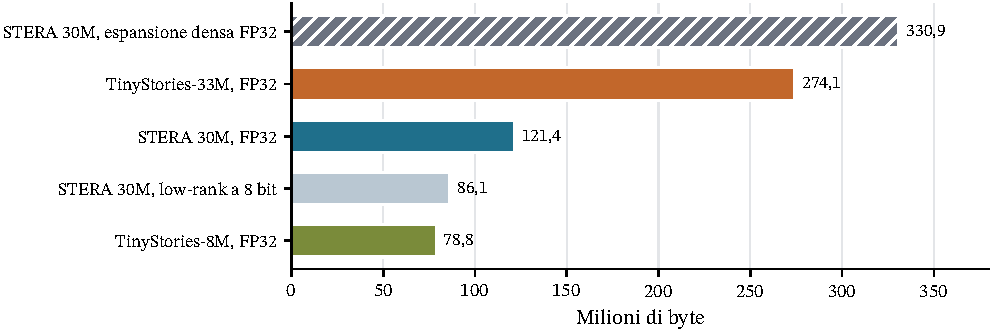
\includegraphics[width=.95\linewidth]{figure/risultati/byte_pesi_stera30m.pdf}
\caption{Byte occupati dai pesi di STERA 30M nelle diverse rappresentazioni, confrontati con i checkpoint TinyStories in FP32 e con l'espansione densa dello stesso modello.}
\label{fig:byte-pesi}
\end{figure}

La \autoref{fig:byte-pesi} ordina le rappresentazioni dalla più grande alla più piccola. In alto, tratteggiata, c'è l'espansione densa di STERA 30M: sono gli stessi pesi scritti come matrici piene, \num{330,9}~MB. La forma compatta degli stessi pesi occupa $121{,}4$~MB, meno della metà di TinyStories-33M ($274{,}1$~MB), e con il low-rank a 8 bit scende a $86{,}1$~MB, vicino a TinyStories-8M ($78{,}8$~MB), che però ha una quota di racconti corretti molto inferiore.

Il $63{,}32\%$ rispetto alla propria espansione densa è il risultato della \autoref{prop:risparmio-modello}: i blocchi RowMask23 garantiscono l'$80{,}61\%$ sulla parte strutturata e il termine low-rank di rango 96 ne consuma la parte restante. Il $55{,}71\%$ rispetto a TinyStories-33M confronta invece due modelli diversi e va letto insieme alla qualità dei racconti (\autoref{sec:risultati-stera30m-tinystories}): STERA 30M occupa meno della metà dei byte con una quota di racconti corretti non significativamente diversa.

Quantizzando a 8 bit i soli fattori $U$ e $V$, il termine low-rank passa da $51{,}5$ a $16{,}2$~MB e il modello da $121{,}385$ a $86{,}097$~MB, il $73{,}98\%$ in meno della propria espansione densa. La matrice densa equivalente cambia dello $0{,}48\%$ in norma e la NLL del $+0{,}007\%$ (\autoref{sec:studio-basso-rango}). Il modello valutato nei confronti di qualità e nei benchmark principali è il compatto FP32; la variante a 8 bit è misurata a parte nella \autoref{sec:rango8-tempi}.

\section{Memoria durante il training}

Durante il training di STERA 30M le matrici vengono espanse temporaneamente per i prodotti con le activation. I due momenti di Adam sono associati ai parametri allenabili della rappresentazione compatta. In FP32, assumendo quattro copie per peso, gradiente e momenti, il conto teorico è di circa 486 MB per STERA 30M. L'analogo conto per gli stessi valori espansi trattati come parametri indipendenti darebbe circa 1.324 MB. Activation, matrici temporanee e workspace incidono separatamente sul picco di training.

\section{Confronto dei due motori dello stesso STERA 30M}
\label{sec:replica-stera-dense}

I due motori MLX/Metal eseguono gli stessi pesi, quelli del checkpoint finale di STERA 30M, sullo stesso Mac, a pesi residenti e precisione FP32. Il percorso compatto usa le coordinate RowMask23. Il percorso Dense carica l'espansione equivalente. Entrambi usano prefill a blocchi, SDPA in decode, batch 1 e KV cache di capacità 512. I sei input contano 256 token ciascuno e l'ordine dei motori viene alternato. La misura è ripetuta in cinque campagne, ciascuna avviata solo quando la media di carico del sistema a un minuto era scesa sotto 1,5, per un totale di 30 coppie di richieste a caldo. In ogni coppia coincidono tutti i 101 ID greedy sia alla prima richiesta sia a caldo, e gli ID sono gli stessi in tutte le campagne.

\begin{table}[htbp]
\centering
\begin{tabular}{lrrr}
\toprule
Motore & TTFT (ms) & Decode (tok/s) & Totale (s) \\
\midrule
STERA 30M Dense & 28,8 & 130,26 & 0,797 \\
STERA 30M compatto & 61,0 & 200,58 & 0,559 \\
\bottomrule
\end{tabular}
\caption{Mediane a caldo su 30 misure appaiate (sei input in cinque campagne). Il caricamento dei pesi è escluso.}
\label{tab:replica-stera-dense}
\end{table}

\begin{figure}[htbp]
\centering
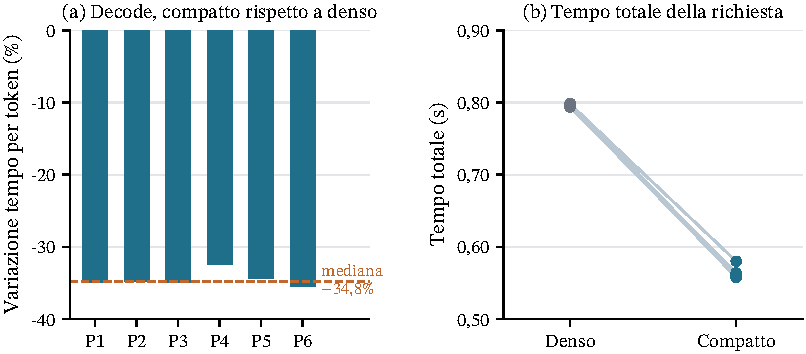
\includegraphics[width=\linewidth]{figure/risultati/decode_appaiato_stera30m.pdf}
\caption{Confronto appaiato fra il motore compatto e il motore denso sugli stessi pesi, per i sei input da 256 token; ogni valore è la mediana delle cinque campagne. (a) Variazione del tempo per token in decode. (b) Tempo totale della richiesta: ogni linea collega le due misure dello stesso input.}
\label{fig:decode-appaiato}
\end{figure}

Nel pannello (a) della \autoref{fig:decode-appaiato} ogni barra è la variazione del tempo per token del motore compatto rispetto al denso su uno dei sei input: tutte le barre sono negative, cioè il compatto è più rapido su ogni input. Nel pannello (b) ogni linea collega il tempo totale della stessa richiesta con i due motori, e tutte scendono passando al compatto. La riduzione mediana appaiata del tempo per passo di decode è del $34{,}8\%$, con riduzioni osservate da $18{,}0\%$ a $39{,}6\%$ sulle 30 coppie; le mediane delle singole campagne sono comprese fra $33{,}7\%$ e $36{,}0\%$. Il Dense emette prima il primo token in tutte le 30 coppie, mentre il compatto impiega meno tempo totale in tutte le 30. Il confronto dei soli payload FP32 vale 121,385 contro 330,885 MB. Questi valori descrivono i pesi, mentre cache, buffer e runtime contribuiscono alla memoria di esecuzione.

\section{Inferenza applicativa: STERA 30M e i due TinyStories}
\label{sec:tre-checkpoint-inferenza}

Riprendiamo i tre checkpoint del confronto di qualità della \autoref{sec:risultati-stera30m-tinystories}. La \autoref{tab:tre-checkpoint-ram} riporta il payload FP32 dei parametri, i tempi e il picco di memoria del processo durante una richiesta con 256 token in ingresso e 100 generati, per due esecuzioni dei riferimenti: con lo stesso motore denso MLX usato per STERA 30M e con il motore standard Transformers su PyTorch/MPS. In entrambe i due TinyStories producono gli stessi token dell'implementazione di riferimento, in ogni campagna. Il picco è il massimo campionato ogni 10 ms durante la richiesta a caldo e include le allocazioni trattenute dal runtime.

\begin{table}[htbp]
\centering
\small
\begin{tabularx}{\linewidth}{Xrrrrr}
\toprule
Modello e motore & Pesi FP32 & TTFT & Decode & Totale & Picco RAM \\
 & (MB) & (ms) & (tok/s) & (s) & (MiB) \\
\midrule
\multicolumn{6}{l}{\emph{Stesso motore MLX}} \\
TinyStories-8M & 78,810 & 13,3 & 311,9 & 0,334 & 511 \\
STERA 30M, compatto & 121,385 & 100,9 & 201,0 & 0,599 & 413 \\
TinyStories-33M & 274,056 & 20,8 & 158,0 & 0,654 & 879 \\
STERA 30M, denso & 330,885 & 29,5 & 130,1 & 0,800 & 569 \\
\midrule
\multicolumn{6}{l}{\emph{Motore standard Transformers su PyTorch/MPS}} \\
TinyStories-8M & 78,810 & 22,9 & 149,8 & 0,691 & \num{1526} \\
TinyStories-33M & 274,056 & 31,7 & 90,6 & 1,136 & \num{1493} \\
\bottomrule
\end{tabularx}
\caption{Inferenza FP32 sul Mac M1: mediane di 15 richieste a caldo (tre input in cinque campagne). Il TTFT di STERA compatto è misurato con il prodotto diretto a blocchi di 16 token; la \autoref{sec:prefill-misure} mostra come ridurlo.}
\label{tab:tre-checkpoint-ram}
\end{table}

Con lo stesso motore, STERA 30M genera più rapidamente di TinyStories-33M, pur avendo sei layer contro quattro e la stessa dimensione, e più lentamente di TinyStories-8M, che esegue circa un quarto delle operazioni per token. Completa la richiesta prima del 33M e della propria forma densa ed è il modello con il picco di memoria più basso. Con il motore standard, i due TinyStories sono più lenti di un fattore fra 1,7 e 2: la differenza fra le due righe dello stesso modello misura il peso del framework, non del modello.

\paragraph{Budget di training.} STERA 30M è addestrato su \num{1529514422} token target, escluso il padding. L'autore di TinyStories-33M \href{https://huggingface.co/roneneldan/TinyStories-33M/discussions/8}{dichiara circa 20 epoche}. Sedici campioni del file ufficiale, tokenizzati con il BPE pubblico, danno una stima di circa 475 milioni di token per passaggio e circa 9,5 miliardi su 20 passaggi. È un ordine di grandezza basato sul tokenizer disponibile; per TinyStories-8M il totale non è documentato. I riferimenti hanno quindi visto un numero di token sensibilmente maggiore di STERA 30M.

\section{Lunghezza dell'ingresso}
\label{sec:contesto-misure}

Le misure precedenti usano 256 token in ingresso. Per verificare se il risultato dipende da questa scelta, gli stessi modelli sono stati misurati con 32, 64, 128, 256 e 384 token in ingresso, sempre con 100 token generati e con lo stesso protocollo di cinque campagne. La \autoref{fig:contesto-prefill} riporta TTFT e decode.

\begin{figure}[htbp]
\centering
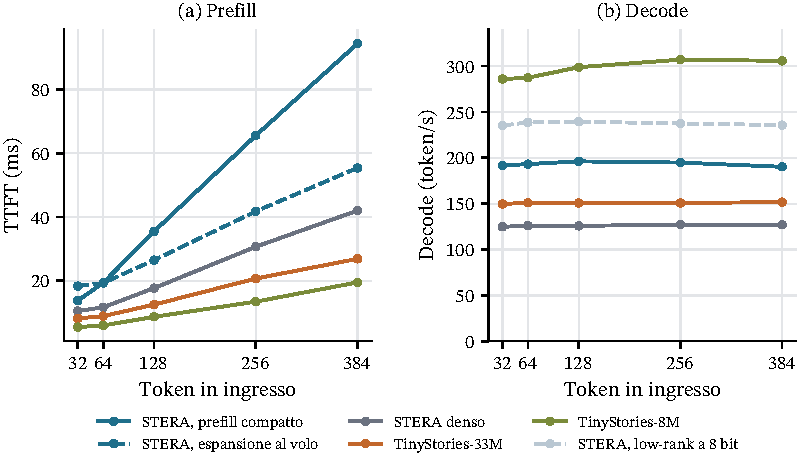
\includegraphics[width=\linewidth]{figure/risultati/contesto_prefill_mlx.pdf}
\caption{TTFT (a) e decode (b) al variare dei token in ingresso, con 100 token generati, sullo stesso motore MLX. Mediane di 15 richieste a caldo per punto.}
\label{fig:contesto-prefill}
\end{figure}

Nella \autoref{fig:contesto-prefill} l'asse orizzontale è il numero di token in ingresso. Il pannello (b) mostra la velocità di generazione: le linee sono quasi orizzontali, cioè il decode non dipende dalla lunghezza dell'ingresso in questo intervallo, e l'ordine dei modelli non cambia mai. TinyStories-8M è il più rapido, seguito da STERA con low-rank a 8 bit, da STERA compatto, da TinyStories-33M e infine dalla forma densa di STERA: per STERA 30M resta fra 191 e 198 token/s e la riduzione del tempo per token rispetto alla forma densa resta fra il $35{,}4\%$ e il $36{,}3\%$. Fino a 484 posizioni il costo dell'attention è piccolo rispetto alla lettura dei pesi, che è la grandezza su cui agisce il formato compatto. Il pannello (a) mostra invece il TTFT, che cresce con la lunghezza dell'ingresso per tutti i modelli. La linea continua di STERA con il prefill compatto è la più ripida: a 384 token impiega $94$~ms contro i $42$~ms della forma densa. La linea tratteggiata, STERA con l'espansione al volo descritta nella \autoref{sec:prefill-misure}, ha una pendenza molto minore e a 384 token scende a $55$~ms.

\section{Elaborazione del prefisso}
\label{sec:prefill-misure}

Nel prefill tutti i token dell'ingresso usano gli stessi pesi e il costo è dominato dal calcolo. Su 256 token, le sole proiezioni richiedono 56~ms con il prodotto diretto sulle coordinate e 19~ms con il prodotto matrice per matrice denso: il kernel compatto, pensato per pochi token alla volta, rilegge coordinate e correzioni per ogni gruppo di token e non sfrutta le unità di calcolo matriciale. Due interventi riducono la differenza:
\begin{itemize}
\item \textbf{dimensione del blocco di token}: con blocchi di 64 token invece di 16, il TTFT su 256 token scende da circa 101 a 66~ms, con gli stessi token generati;
\item \textbf{espansione al bisogno}: per ogni layer si ricostruisce con un kernel dedicato la parte strutturata delle sei proiezioni, esattamente uguale bit per bit a quella del training, si eseguono i prodotti densi su tutti i token e si rilasciano le matrici prima del layer successivo; il termine low-rank resta fattorizzato. Il decode resta sul prodotto diretto.
\end{itemize}

\begin{table}[htbp]
\centering
\small
\begin{tabular}{rrrrr}
\toprule
Token in ingresso & Prodotto diretto & Espansione al bisogno & Espansione, rango 8 bit & Denso \\
\midrule
32 & 13,8 & 18,3 & 18,0 & 10,5 \\
64 & 19,3 & 19,3 & 19,6 & 11,6 \\
128 & 35,5 & 26,5 & 28,7 & 17,7 \\
256 & 65,6 & 41,8 & 42,0 & 30,7 \\
384 & 94,4 & 55,4 & 54,9 & 42,0 \\
\bottomrule
\end{tabular}
\caption{TTFT di STERA 30M in millisecondi, con le diverse strategie di prefill. Prodotto diretto a blocchi di 64 token; mediane di 15 richieste a caldo.}
\label{tab:prefill-strategie}
\end{table}

L'espansione al bisogno riduce il TTFT di circa il $40\%$ per gli ingressi da 256 token in su, con gli stessi token generati e senza aumentare il picco di memoria, perché le matrici espanse di un layer occupano circa 54~MB e vengono rilasciate subito. Per ingressi molto brevi il costo fisso dell'espansione non è compensato e conviene il prodotto diretto: la soglia fra le due strategie è intorno ai 64 token. Il motore denso resta più rapido nel TTFT, ma il divario si dimezza.

\section{Low-rank a 8 bit}
\label{sec:rango8-tempi}

Il termine low-rank quantizzato a 8 bit può restare in quel formato anche durante l'esecuzione: il motore moltiplica direttamente i fattori a 8 bit, senza riconvertirli in FP32. Misurato con lo stesso protocollo, su 256 token in ingresso, il decode passa da $198{,}9$ a $241{,}9$ token/s, con una riduzione del tempo per token del $17{,}8\%$ (da $-10{,}1\%$ a $-24{,}5\%$ sulle 15 coppie), mentre il TTFT non cambia ($63{,}4$ e $65{,}4$~ms). Su due input su tre i token generati coincidono con quelli del modello FP32 per tutti i 101 passi, sul terzo si separano al passo 37, coerentemente con una NLL praticamente invariata. La memoria attiva della GPU scende da 137 a 104~MiB; il picco dell'intero processo resta invece di circa 433~MiB, dominato dal runtime e dai buffer.

Combinando espansione al bisogno nel prefill e low-rank a 8 bit, STERA 30M completa una richiesta con 256 token in ingresso e 100 generati in $0{,}47$~s, contro $0{,}82$~s della propria forma densa con lo stesso motore.

\section{Un modello delle dimensioni di Qwen3.5-9B: STERA F10}
\label{sec:qwen-f10-ssd}

Le misure precedenti riguardano un modello piccolo, che entra comodamente in memoria. Per vedere che cosa cambia quando i pesi si avvicinano al limite del dispositivo confrontiamo due modelli di taglia simile: Qwen3.5-9B, un modello pubblico addestrato, e STERA F10, un modello fittizio costruito con la parametrizzazione STERA.

\paragraph{Che cosa è F10.} F10 è STERA 30M allargato dieci volte: hidden size \num{7680}, 160 head, feed-forward \num{30720}, sei layer e lo stesso vocabolario, per \num{898109280} coordinate e \num{4633067520} valori nella forma densa equivalente. È generato da uno script deterministico a partire dal checkpoint finale di STERA 30M: ogni blocco nuovo copia le coordinate di un blocco addestrato, divise per dieci e leggermente perturbate, così che ogni blocco abbia coordinate proprie. Il file generato è identico bit per bit su ogni macchina ed è identificato dalla sua impronta. \textbf{F10 non è addestrato}: serve solo come termine di confronto delle risorse necessarie all'esecuzione, e le sue generazioni non hanno valore linguistico. È eseguito con il motore compatto del \autoref{cap:capitoli/04d-motore}.

\paragraph{Soglia di memoria.} I pesi compatti di F10 occupano \num{4002707952} byte, cioè 3,73~GiB. La sua forma densa occuperebbe 17,32~GiB, più dei 16~GiB del dispositivo, e Qwen3.5-9B in BF16 ne occupa 16,68 (\autoref{fig:soglia-ram-f10}).

\begin{figure}[H]
\centering
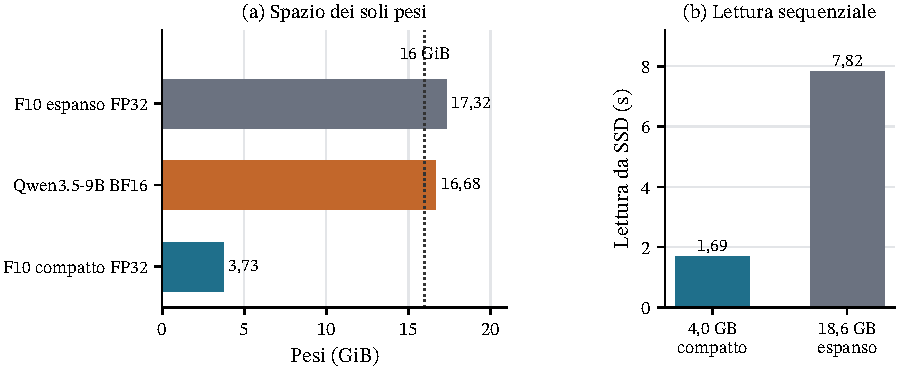
\includegraphics[width=\linewidth]{figure/risultati/soglia_ram_m1.pdf}
\caption{(a) Spazio occupato dai soli pesi del modello fittizio F10 in forma compatta ed espansa e di Qwen3.5-9B in BF16, rispetto ai 16~GiB di memoria del dispositivo. (b) Tempo mediano di lettura sequenziale dall'SSD dei due volumi del modello fittizio F10.}
\label{fig:soglia-ram-f10}
\end{figure}

Nel pannello (a) della \autoref{fig:soglia-ram-f10} la linea tratteggiata verticale è la memoria del dispositivo. Si osserva che la forma compatta di F10 sta ampiamente sotto la soglia, mentre la sua espansione densa e Qwen3.5-9B la superano: per eseguirli i pesi andrebbero letti dal disco. Il pannello (b) mostra il costo di quella lettura: rileggere dall'SSD il volume denso richiede 7,82~s, contro 1,69~s per il volume compatto.

\paragraph{Decode al variare del contesto.} La \autoref{tab:f10-contesto}, subito sotto, riporta il decode di F10 con i pesi residenti al variare della lunghezza del contesto, cioè del numero di posizioni presenti nella KV cache. È lo scenario di una conversazione o di un agente il cui contesto si è accumulato fino a quella lunghezza. Fino a \num{16000} token la cache è in FP32; a \num{32000} token è misurata sia in FP32 sia in FP16, e a \num{64000} token solo in FP16, l'unica precisione con cui entra in memoria.

\begin{table}[H]
\centering
\small
\begin{tabular}{rlrrr}
\toprule
Contesto (token) & KV cache & Decode (token/s) & Tempo per token (ms) & Memoria (GiB) \\
\midrule
128 & FP32 & 12,6 & 79 & 4,0 \\
512 & FP32 & 12,3 & 81 & 4,3 \\
\num{2000} & FP32 & 11,5 & 87 & 4,3 \\
\num{8000} & FP32 & 9,2 & 109 & 5,3 \\
\num{16000} & FP32 & 7,4 & 136 & 6,7 \\
\num{32000} & FP32 & 5,1 & 196 & 9,6 \\
\num{32000} & FP16 & 6,0 & 166 & 6,7 \\
\num{64000} & FP16 & 3,9 & 257 & 9,6 \\
\bottomrule
\end{tabular}
\caption{Decode del modello fittizio STERA F10 con pesi residenti al variare del contesto. Mediane di tre esecuzioni a sistema scarico, 24 token ciascuna; la memoria è il picco occupato sulla GPU da pesi e KV cache.}
\label{tab:f10-contesto}
\end{table}

Come mostra la \autoref{tab:f10-contesto}, fino a \num{2000} token il tempo per token resta intorno agli 80~ms, perché è dominato dalla lettura dei pesi. Oltre, cresce con il contesto, perché a ogni token l'attention deve leggere tutte le posizioni della cache: a \num{32000} token il decode scende a circa 5 token/s e a \num{64000} a circa 4. La memoria cresce nello stesso modo, da 4,0 a 9,6~GiB, e resta sempre dentro i 16~GiB del dispositivo. La cache in FP16 dimezza lo spazio della cache e rende il decode più rapido, perché ci sono meno byte da leggere.

\paragraph{Limiti della misura e sua affidabilità.} La misura ha due limiti. La KV cache è riempita direttamente con valori di prova, invece che dall'elaborazione di un prompt reale, quindi il TTFT a contesto lungo non è misurato. F10 non è addestrato, quindi la misura non dice nulla sulla qualità a contesto lungo. La misura resta affidabile per ciò che descrive, cioè memoria e tempo per token: le operazioni di un passo di decode dipendono dal numero di posizioni nella cache e non dai valori che contiene, e una prova di controllo in cui il modello riempie la cache generando \num{8000} token ha dato, allo stesso stato termico del dispositivo, un tempo per token entro il $4\%$ di quello misurato. Tutte le misure sono eseguite sulla GPU del dispositivo reale, con il modello letto dal file generato.

\paragraph{Qwen3.5-9B con i layer letti dal disco.} Per verificare una strategia reale di esecuzione oltre la memoria è stato eseguito il decoder di Qwen3.5-9B, con pesi BF16, runtime SWLP su PyTorch/MPS, batch 1 e lettura dei layer dall'SSD. Embedding e output head restano in memoria, mentre i blocchi attraversano una finestra di caricamento e prefetch. Il modello è addestrato, ma qui interessa solo il suo costo di esecuzione su memoria limitata: non è un riferimento per la qualità narrativa di STERA 30M.

\begin{table}[H]
\centering
\small
\begin{tabular}{rrrrr}
\toprule
Input (token) & TTFT (s) & Decode (tok/s) & Picco processo (GiB) & Letture SSD (GB) \\
\midrule
256 & 12,06 & 0,153 & 7,63 & 57,15 \\
\num{4096} & 95,55 & 0,147 & 7,45 & 154,50 \\
\bottomrule
\end{tabular}
\caption{Qwen3.5-9B in BF16 con SWLP, una prova per condizione, quattro token generati, prefetch attivo. Il decode comprende i tre passi successivi al primo; letture e picco includono il caricamento.}
\label{tab:qwen-swlp}
\end{table}

Con 256 token di input, una prova separata disattiva il prefetch e riporta 0,126 token/s nel decode, contro 0,153 con prefetch. Sono singole prove, a causa della loro durata, e non forniscono un intervallo sulla variabilità di esecuzione.

\paragraph{Confronto dei due regimi.} La \autoref{tab:f10-qwen}, subito sotto, mette a confronto i due modelli nelle condizioni misurate.

\begin{table}[H]
\centering
\small
\begin{tabular}{lrr}
\toprule
& STERA F10 compatto & Qwen3.5-9B con SWLP \\
\midrule
Pesi & 3,73~GiB in FP32 & 16,68~GiB in BF16 \\
Dove stanno i pesi & tutti in memoria & layer letti dal disco \\
Modello addestrato & no & sì \\
Decode, contesto breve (token/s) & 12,6 & 0,153 \\
Tempo per token, contesto breve & 0,079~s & 6,5~s \\
Decode a circa 4.000 token (token/s) & 9,2 (a \num{8000}) & 0,147 (a \num{4096}) \\
\bottomrule
\end{tabular}
\caption{STERA F10 compatto e Qwen3.5-9B a confronto. Modelli, precisioni e runtime sono diversi: il confronto descrive due regimi di memoria, pesi residenti contro pesi letti dal disco, non la velocità a parità di modello.}
\label{tab:f10-qwen}
\end{table}

F10 genera circa un token ogni 80~ms perché tutti i suoi pesi stanno in memoria; Qwen3.5-9B, che non ci sta, impiega circa 6,5~s per token perché a ogni token rilegge i layer dal disco. La stessa sorte toccherebbe all'espansione densa di F10: la sola lettura dei suoi 18,6~GB dall'SSD richiede 7,82~s, cioè circa 0,13 token/s se il volume andasse riletto a ogni token. Il risultato non è un confronto di velocità fra modelli, ma la conferma della motivazione della tesi: con la parametrizzazione STERA un modello di questa taglia resta in memoria, dove la sua forma densa non ci starebbe.

\section{Sintesi}

Sullo stesso STERA 30M, il motore che applica le proiezioni direttamente alle coordinate riduce del $34{,}8\%$ il tempo mediano per token in decode rispetto al motore con matrici dense equivalenti, producendo gli stessi token, e il vantaggio resta costante fra 32 e 384 token in ingresso. Il motore denso resta più rapido nel TTFT; l'espansione al bisogno delle matrici nel prefill dimezza il divario. Con lo stesso motore, STERA 30M genera più rapidamente di TinyStories-33M e con il picco di memoria più basso dei modelli misurati. I pesi compatti occupano 121,385~MB in FP32, il $63{,}32\%$ in meno della propria espansione densa; quantizzando a 8 bit il termine low-rank scendono a 86,097~MB ($-73{,}98\%$) e il decode diventa più rapido del $17{,}8\%$. A scala maggiore, il modello fittizio STERA F10, di taglia simile a Qwen3.5-9B, resta interamente in memoria su un dispositivo da 16~GiB con contesti fino a \num{64000} token misurati, a circa 12~token/s con contesto breve e 4~token/s a \num{64000} token; la sua forma densa e Qwen3.5-9B superano la memoria già con i soli pesi, e Qwen3.5-9B, che legge i layer dal disco, genera circa 0,15~token/s.
